\subsubsection{Infinite Horizon}
\begin{frame}{\subsecname: \subsubsecname}
    \begin{figure}
        \centering
        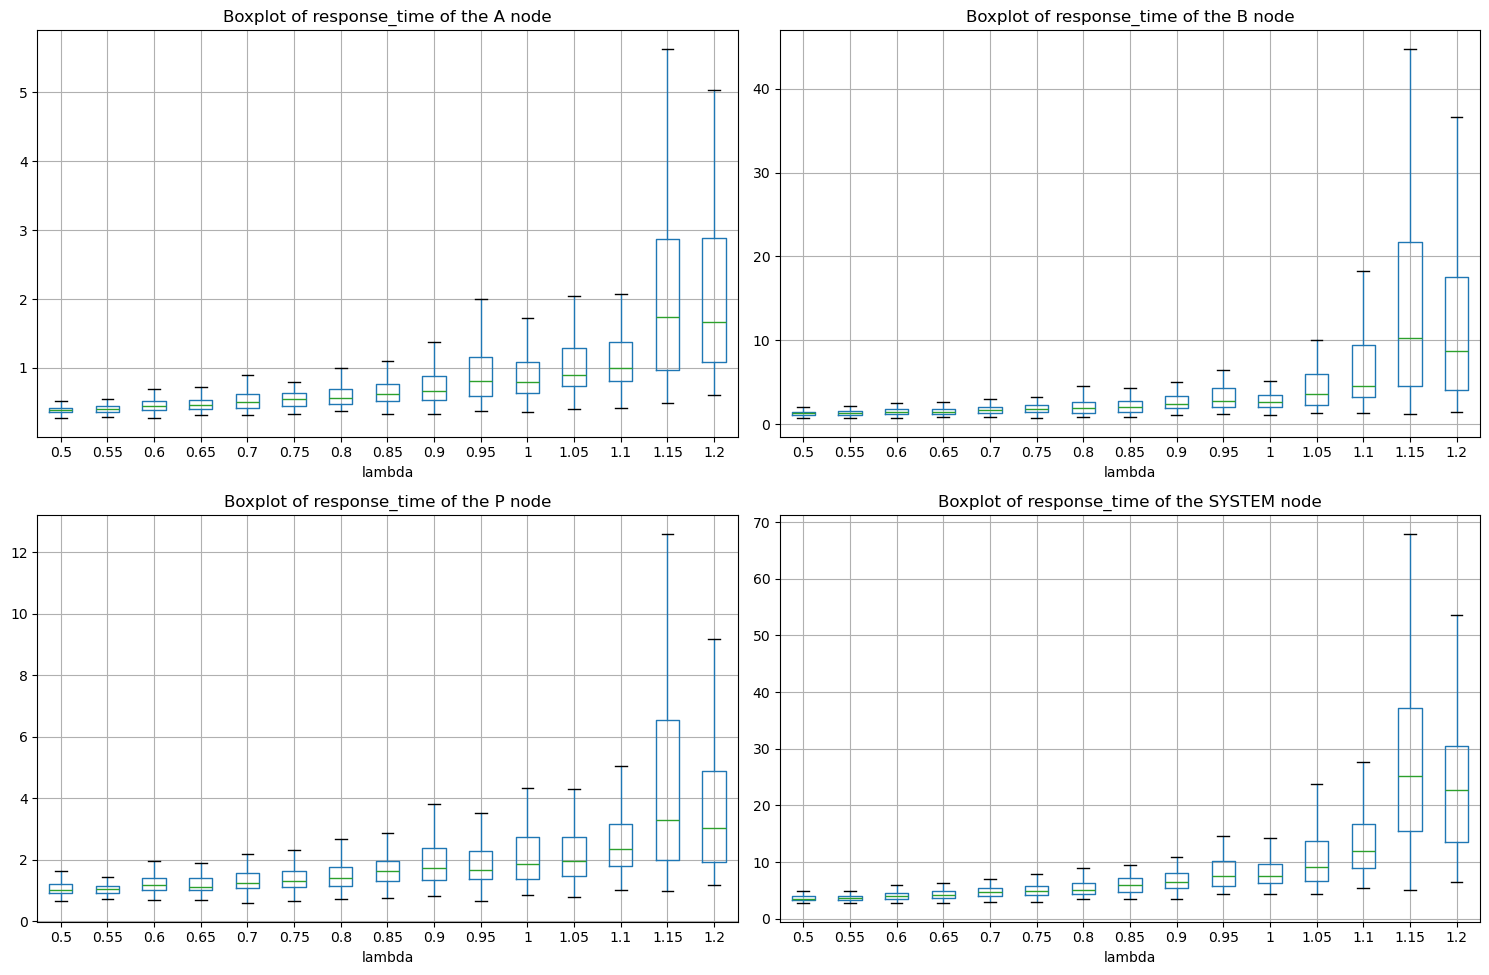
\includegraphics[width=0.75\linewidth]{figs/results/obj2/simulation/obj2_boxplot_rtime.png}
        \caption{Distribuzione del Tempo di Risposta medio dei risultati sperimentali dell’obbiettivo 2}
        \label{fig:enter-label}
    \end{figure}
\end{frame}

\subsubsection{Finite Horizon}
\begin{frame}{\subsecname: \subsubsecname}
    \begin{figure}
        \centering
        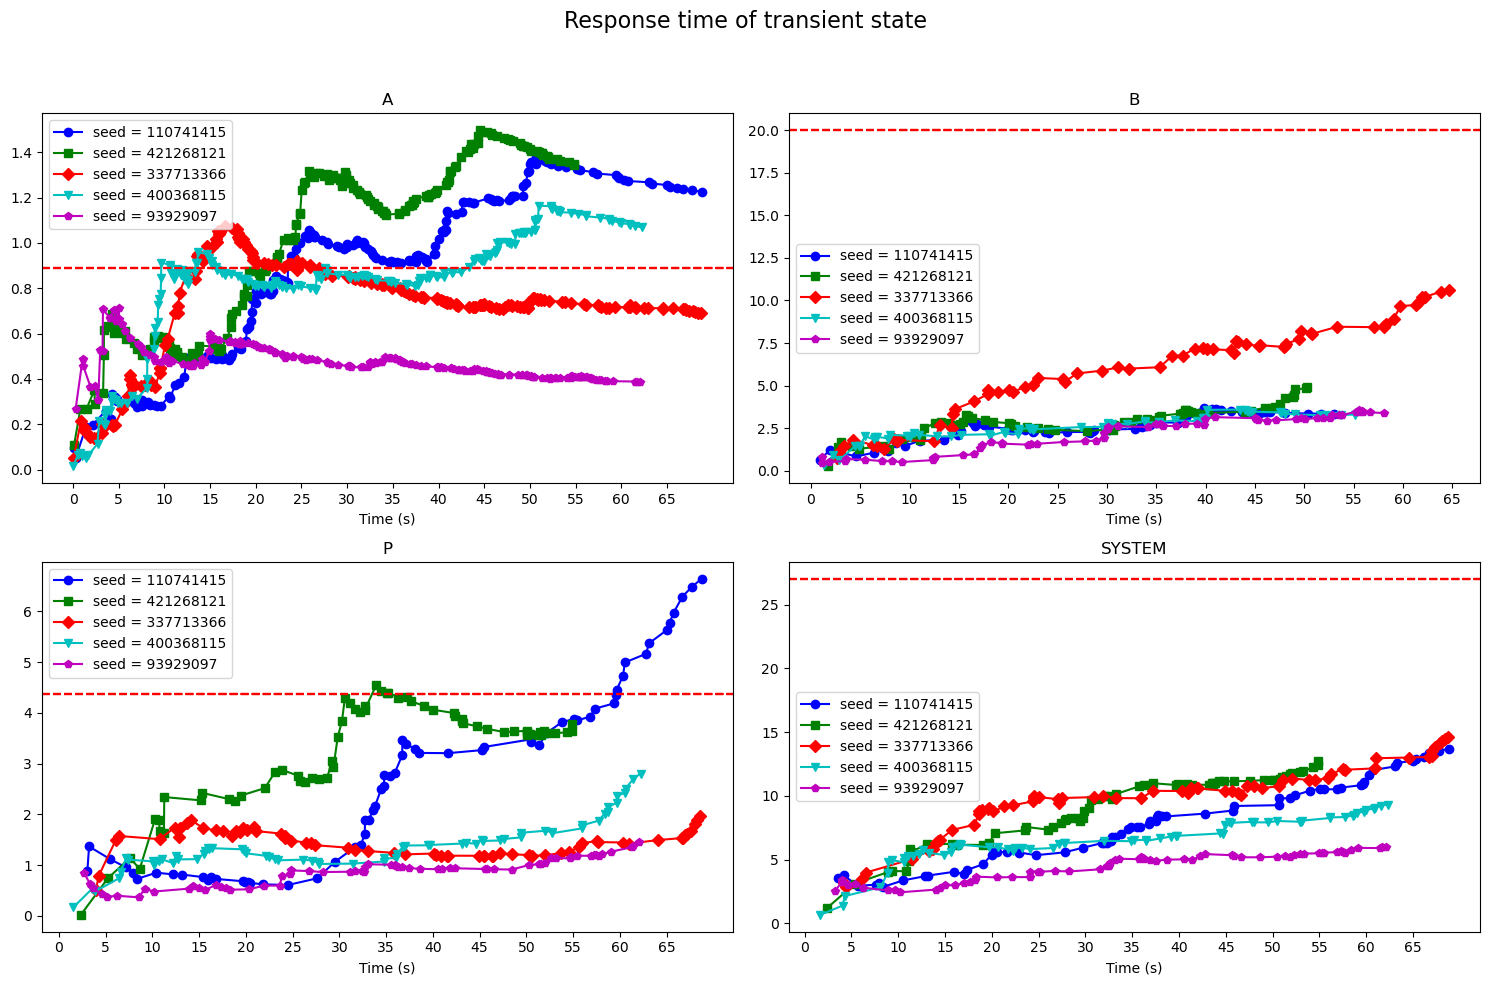
\includegraphics[width=0.75\linewidth]{figs/appendices/transient/obj2-transient-rtime-analitycal.png}
        \caption{Tempo di risposta per l’obiettivo 2 in funzione del tempo di simulazione nello stato transiente del sistema con un rate di arrivi 1.2 $job/s$ al variare del seed}
        \label{fig:enter-label}
    \end{figure}
\end{frame}

\subsubsection{Verification}
\begin{frame}{\subsecname: \subsubsecname}
\begin{figure}
    \centering
    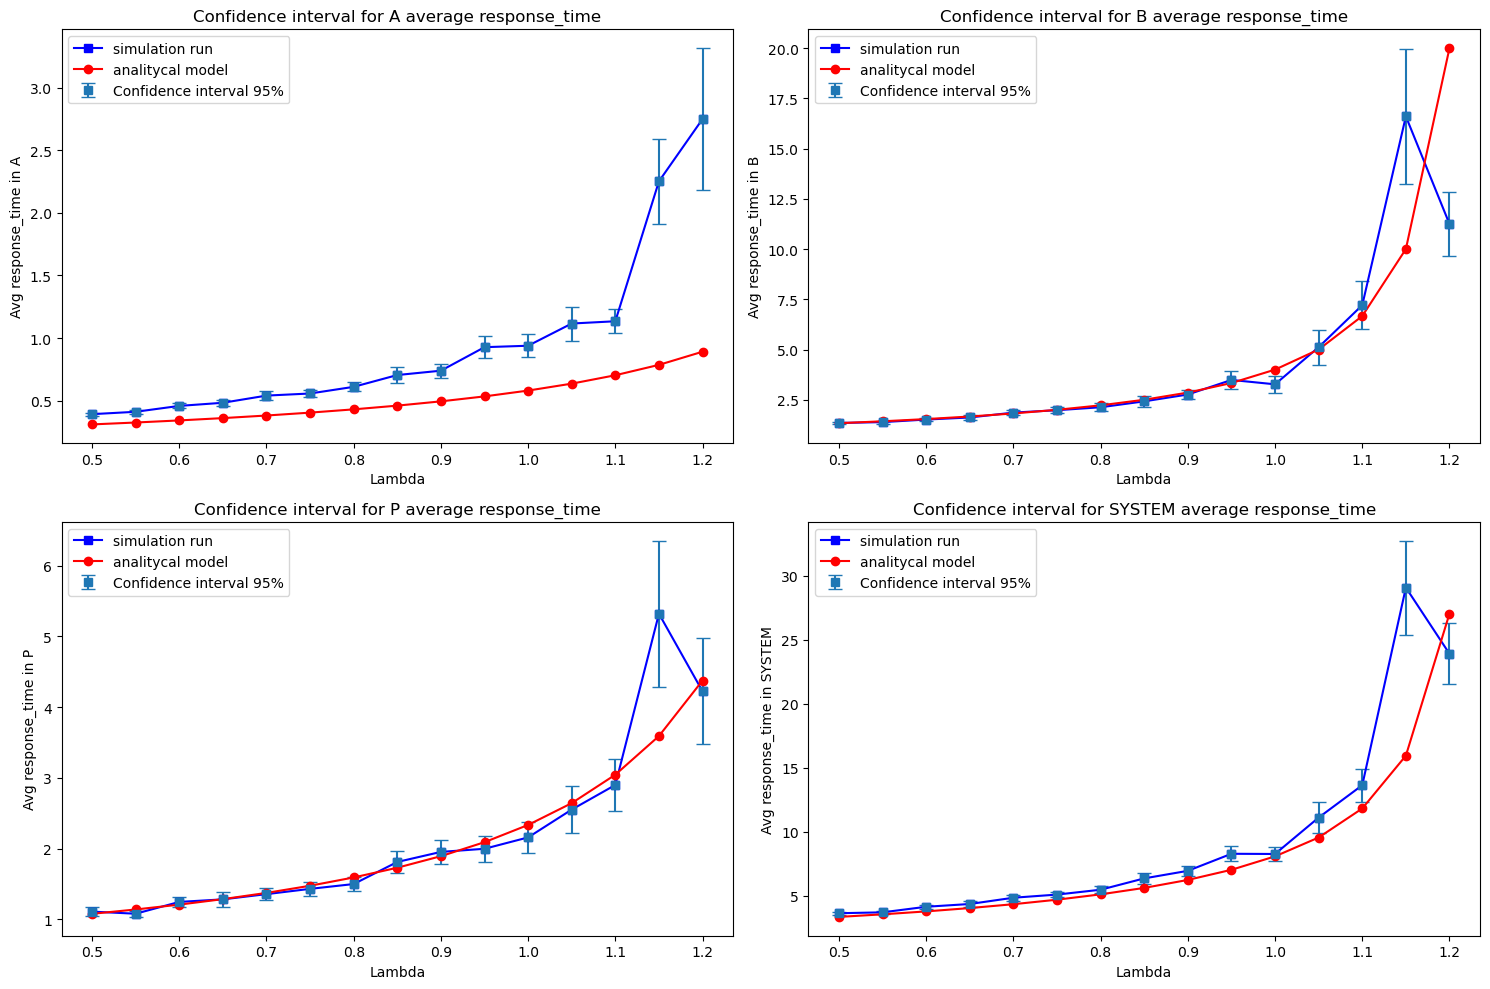
\includegraphics[width=0.75\linewidth]{figs/results/obj2/verification/obj2_lineplots_rtime.png}
    \caption{ Confronto tra valori medi della simulazione e del modello analitico del Tempo di Risposta per l’Obiettivo 2.}
    \label{fig:enter-label}
\end{figure}   
\end{frame}

\subsubsection{Validation}
\begin{frame}{\subsecname: \subsubsecname}
\begin{figure}
    \centering
    \begin{subfigure}{0.49\linewidth}
        \centering
        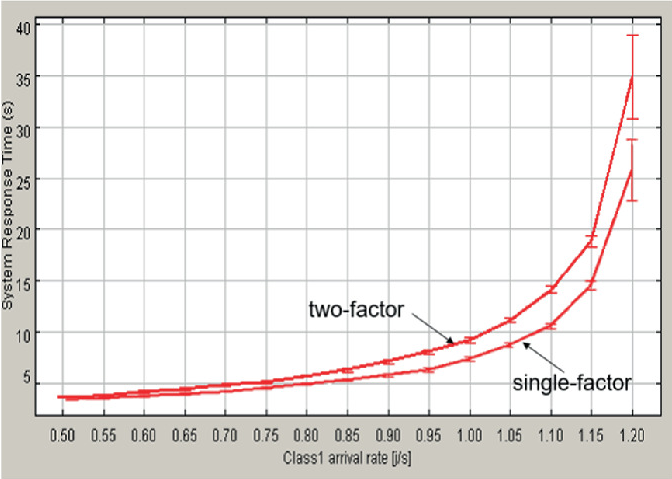
\includegraphics[width=1\linewidth]{figs/results/obj2/validation/casestudy_system_rtime.png}
        \caption{Case Study \citep{DBLP:books/sp/Serazzi24}}
        \label{fig:Single_VS_Two_FA_Perfomance_Comparison_population}
    \end{subfigure}
    % \hfill
    \begin{subfigure}{0.49\linewidth}
        \centering
        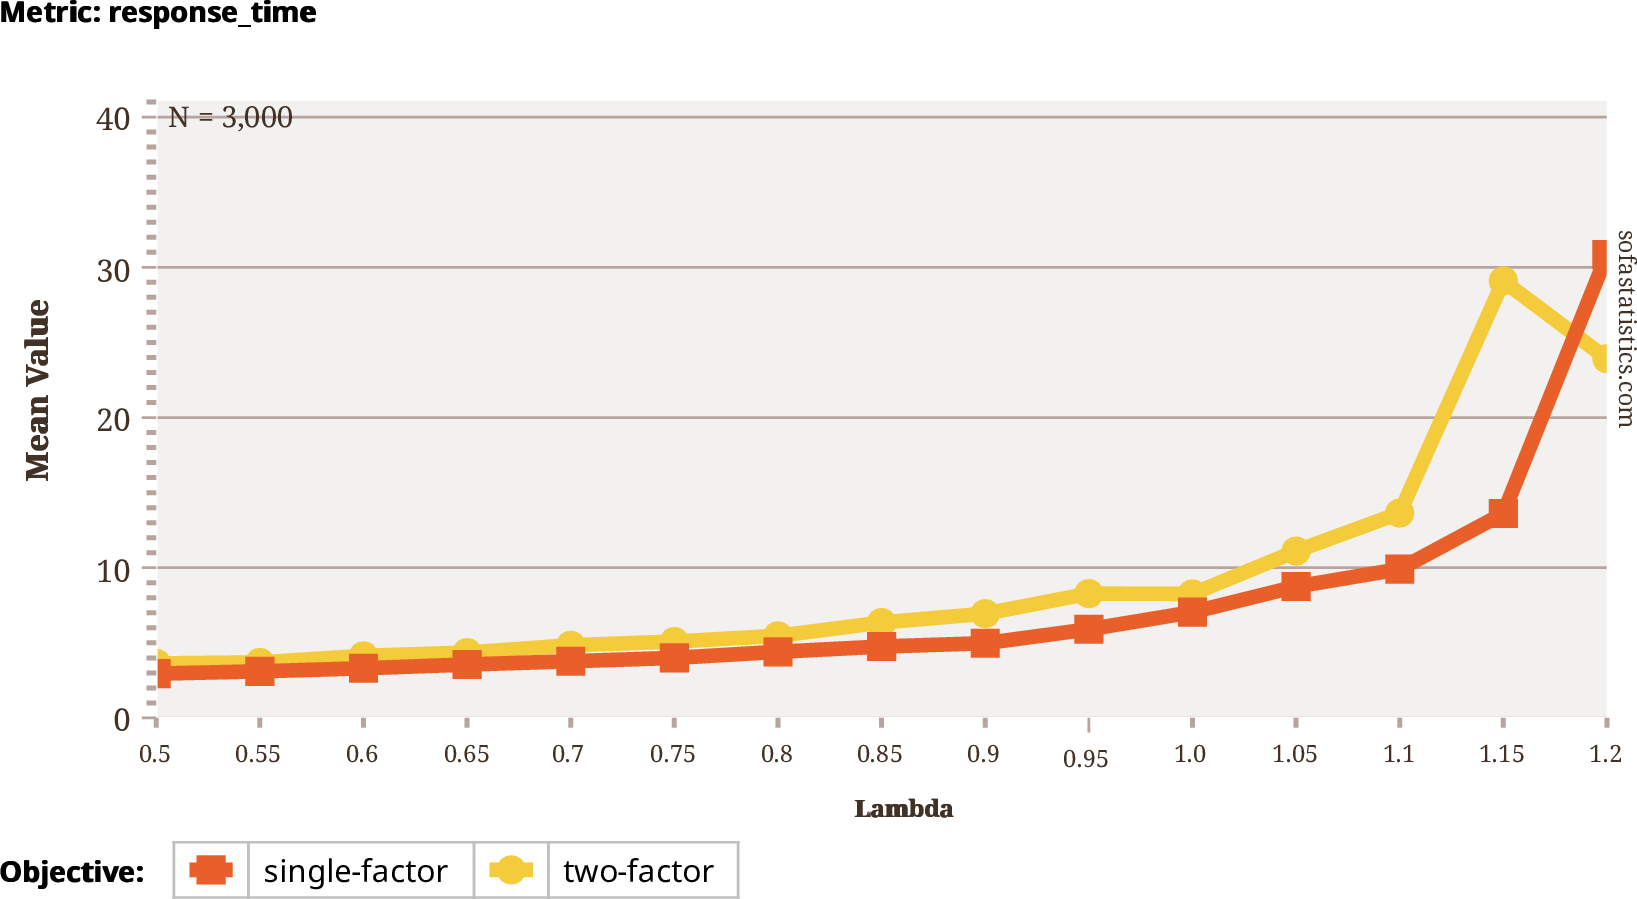
\includegraphics[width=1\linewidth]{figs/results/obj2/validation/single_VS_Two_FA_Perfomance_Comparison_rtime.png}
        \caption{Simulazione}
        \label{fig:Single_VS_Two_FA_Perfomance_Comparison_rtime}
    \end{subfigure}
    % \hfill
    \caption{Tempo di Risposta medi del sistema in funzione del rate di arrivi esterni nel caso con e senza 2FA.}
    \label{fig:Single_VS_Two_FA_Perfomance_Comparison}
\end{figure}
\end{frame}
